\section{Introduction}
\subsection{LBGB au sein du Genoscope et du CEA}
Le Genoscope (CNS) a été créé en 1996 pour participer au projet mondial de séquençage du génome humain (\emph{Human Genome Project}) qui à débuté en 1990 et s'est terminé en 2003. Il a notament participé au séquençage du chromosome 14. Le Genoscope est impliqué dans le développement de programme de génomique en France dans le cadre du projet France génomique. Aujourd'hui les projets phares du Genoscope sont les projets \textbf{Tara} (\emph{Pacific}, Océans, \emph{Artic} ...), qui ont pour objectifs l'étude des écosystèmes marins ; Le projet \textbf{ERGA}, dont l'objectif est de créer une base de données de références de haute qualité des génomes d'espèces européennes.

\begin{minipage}{0.45\textwidth}
\begin{figure}[H]
    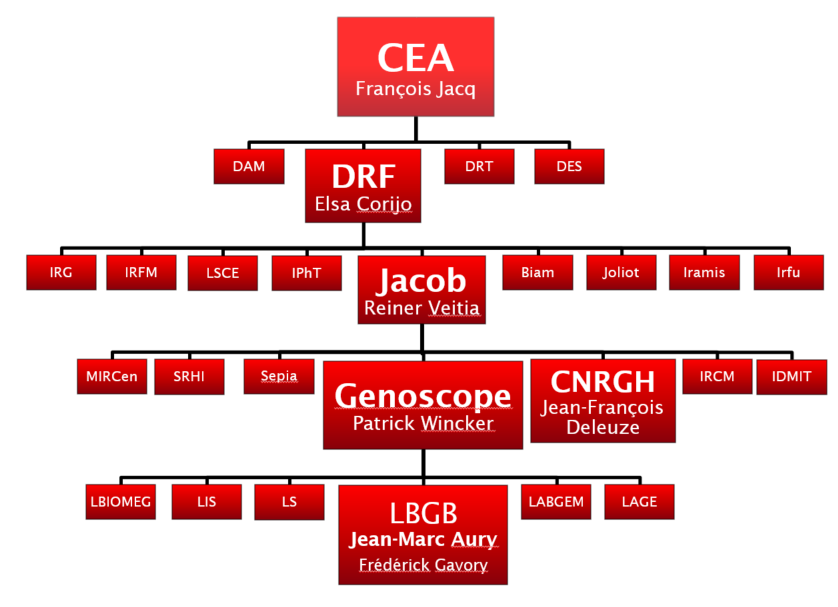
\includegraphics[width=1.1\textwidth]{img/organigramme.png}
    \caption{Organigramme situant l’équipe du LBGB au sein du Genoscope et du CEA}
    \label{organigramme_LBGB}
\end{figure}
\end{minipage} 
\hfill
\begin{minipage}{0.45\textwidth}
    Le Laboratoire de Bioinformatique pour la Génomique et la Biodiversité (\textbf{LBGB}) dirigé par Jean-Marc Aury, fait partie du Genoscope qui est une composante de l'institut de biologie François Jacob (\textbf{IBFJ}) de la direction de la recherche fondamentale (\textbf{DRF}) du Commissariat à l'Énergie Atomique et aux Énergies Alternatives (\textbf{CEA}), qui a été fondé le 18 octobre 1945 par Charles de Gaulle. L'intégration du genoscope au CEA a été réalisée en 2007, et en 2017 il devient une composante de l'IBFJ.
\end{minipage}

\subsection{Contexte et missions du LBGB}
Les missions qui sont confiées au LBGB sont de réaliser le contrôle qualité des données de séquences issues des différents séquenceurs, d'effectuer l'assemblage\footnote{Reconstruction d'un génome à partir de fragments de ce dernier} des séquences et l'annotation\footnote{Documenter le plus exhaustivement possible les informations de l'assemblage permmettant de prédire la fonction d'une molécule} des génomes, dans l'objectif de mettre à disposition des laboratoires collaborateurs les données avec un premiers niveau da valorisation. Le laboratoire est divisé en plusieurs groupes de travail. Le groupe \og production \fg{} (dont je fais partie), le groupe \og assemblage \fg{}, le groupe \og annotation \fg{} et le groupe \og évaluation des technologies de séquençage \fg{}.

Les missions du groupe de \og production \fg{} sont de tester des logiciels tiers, de développer et maintenir des scripts utilisant ces logiciels pour gérer efficacement la prise en charge des données en sortie de séquençeur. Cette prise en charge peut répondre à une demande de la production et des laboratoires du Genoscope et du CNRGH, mais aussi pour des laboratoires extérieur. L'objectif principale est la mise en place et le maintient de pipelines automatisant l'ensemble. Le groupe s'appuie sur un travail de vielle et d'évaluation technologique pour chacune de ses missions. 


\subsection{Présentation du workflow NGS}
\begin{minipage}{0.45\textwidth}
	\begin{figure}[H]
		\centering
		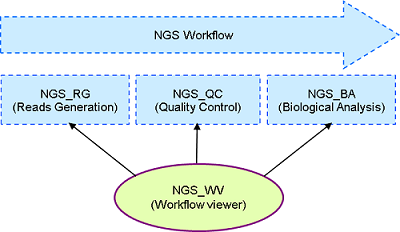
\includegraphics[width=1\textwidth]{img/Workflow.png}
		\caption{\footnotesize{Workflow de génération, de contrôle qualité et d’analyse biologique des fastq}}
		\label{worflow-genoscope}
	\end{figure}
\end{minipage}
\hfill
\begin{minipage}{0.45\textwidth}
	Le workflow NGS est composé de trois pipelines pour les technologies Illumina et Oxford Nanopore. Le premier (ngs\_rg\footnote{\emph{Next Generation Sequencing - reads generation}}), permet la génération des reads\footnote{Lecture d'une séquence par un séquenceur d'un fragments d'ADN} et des fichiers de séquences correspondant aux échantillons. Le second (ngs\_qc\footnote{\emph{Next Generation Sequencing - quality control}}), permet de réaliser leurs contrôle qualité. Le dernier (ngs\_ba\footnote{\emph{Next Generation Sequencing - biological analysis}}), permet de faire les analyses biologiques inter-échantillons (\emph{readset})\footnote{Un lot de séquences est une instance de séquences (ou reads) d'un échantillon}. 
\end{minipage}\\[0.1cm]

Ces trois pipelines sont automatisés dans le workflow et permettent de réaliser la distribution des données de séquençage, par projet, échantillons, runs\footnote{Séquençage d'un ou plusieurs échantillons sur un séquenceur} et technologies de séquençage. Ils réalisent aussi le nettoyage, l'analyse de ces fichiers et mettent à jour la base de données de référence NGL. Les trois pipelines du workflow NGS sont monitorés par NGS \emph{Worqflow Viewer} (NGS\_WV), qui est une application web permettant de surveiller l'avancement des pipelines pour les runs pris en charge par le NGS-workflow.

\subsection{La technologie MGI}
Le genoscope et le CNRGH ont récement fait l'aquisition de séquenceurs MGI (2 DNBSEQ-G400 et 1 DNBSEQ-T7).

\begin{minipage}{0.45\textwidth}
    \begin{figure}[H]
        \centering
        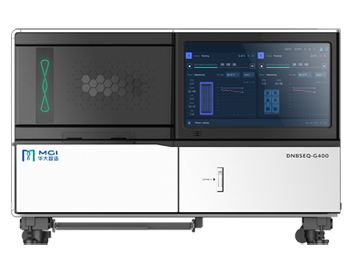
\includegraphics[width=0.5\textwidth]{img/MGI_G400.jpg}\\
        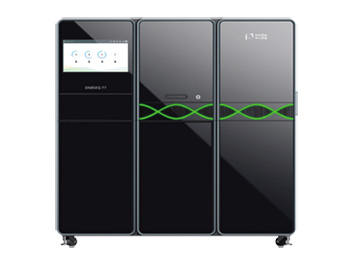
\includegraphics[width=0.5\textwidth]{img/MGI_T7.jpg}
        \caption{\footnotesize{Sequenceurs DNBSEQ-G400 (en haut) et DNBT7 (en bas) de MGI \href{https://en.mgi-tech.com/products/}{https://en.mgi-tech.com/products/}}}
        \label{seq-MGI}
    \end{figure}
\end{minipage} 
\hfill
\begin{minipage}{0.45\textwidth}
	\begin{figure}[H]
        \centering
        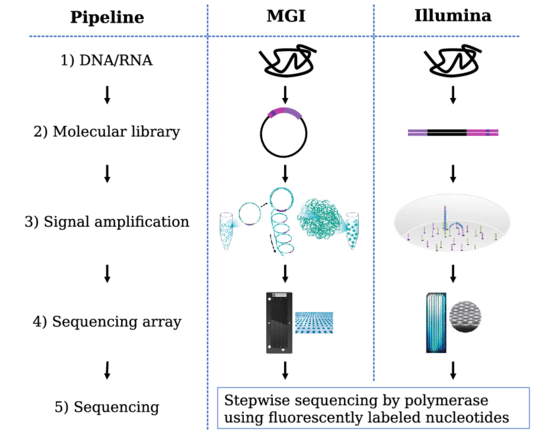
\includegraphics[width=1\textwidth]{img/MGI_vs_Illumina.png}
        \caption{\footnotesize{Différences entre Illumina et MGI de technologie NGS}}
        \label{fig-Illu-vs-MGI}
    \end{figure}
\end{minipage}\\\\

    Il s'agit de séquenceurs à haut débit et très haut débit, dont les principales différences entre MGI et Illumina sont dans la création des librairies\footnote{Collection de fragment d'ADN issue du génome complet d'un organisme ou plusieurs organismes (méta-génomique) et clonés dans un vecteur (le plus souvanet dans des plasmides)} et la méthode d'amplification d'ADN. Les librairies sont double brins circulaire pour MGI, alors que pour Illumina elle est double brins linéaire. L'amplification ADN est réalisée en solution et forme des DNB (\emph{DNA-nanoballs}\footnote{Nanobilles d'ADN générées par la réplication de l'ADN circulaire}), puis déposée sur la Flowcell\footnote{Lame d'absorbtion des fragments d'ADN et cuve réacteur du séquençage} pour MGI, alors que pour Illumina elle est réalisée après immobilisation sur les Flowcell.

\begin{table}[H]
\begin{tabular}{ |p{5cm}||r|r|r|r| }
    \hline
    \multicolumn{5}{|c|}{Sequencers specifications} \\\hline
    & \footnotesize{DNBSEQ-G400} & \footnotesize{DNBSEQ-T7} & \footnotesize{HiSeq 4000} & \footnotesize{NovaSeq 6000} \\\hline\hline
    Max Number of Flow Cells & 2 & 4 & 2 & 2 \\\hline
    Max Lane/Flow Cell & 4 & 1 & 4 & 4 \\\hline
    Run Time & $\sim$ 14-37 h & $\sim$ 20-30 h & $\sim$ 24-84 h & $\sim$ 13-44 h \\\hline
    \textbf{Data ouput/Run} & 0.27-1.4 Tb & 1-6 Tb & 0.9-1.8 Tb & 1-6 Tb \\\hline
    Max Reads/Run & 1.8 billions & 5 billions & 10 billions & 20 billions \\\hline
    Max Read Length & 2 $\times$ 200 bp & 2 $\times$ 150 bp & 2 $\times$ 150 bp & 2 $\times$ 250 bp \\\hline
\end{tabular}
    \caption{Spécification des séquenceurs}
    \label{spe-seq}
\end{table}
